\documentclass[]{article}
\usepackage{lmodern}
\usepackage{amssymb,amsmath}
\usepackage{ifxetex,ifluatex}
\usepackage{fixltx2e} % provides \textsubscript
\ifnum 0\ifxetex 1\fi\ifluatex 1\fi=0 % if pdftex
  \usepackage[T1]{fontenc}
  \usepackage[utf8]{inputenc}
\else % if luatex or xelatex
  \ifxetex
    \usepackage{mathspec}
  \else
    \usepackage{fontspec}
  \fi
  \defaultfontfeatures{Ligatures=TeX,Scale=MatchLowercase}
\fi
% use upquote if available, for straight quotes in verbatim environments
\IfFileExists{upquote.sty}{\usepackage{upquote}}{}
% use microtype if available
\IfFileExists{microtype.sty}{%
\usepackage{microtype}
\UseMicrotypeSet[protrusion]{basicmath} % disable protrusion for tt fonts
}{}
\usepackage[margin=1in]{geometry}
\usepackage{hyperref}
\hypersetup{unicode=true,
            pdfborder={0 0 0},
            breaklinks=true}
\urlstyle{same}  % don't use monospace font for urls
\usepackage{graphicx,grffile}
\makeatletter
\def\maxwidth{\ifdim\Gin@nat@width>\linewidth\linewidth\else\Gin@nat@width\fi}
\def\maxheight{\ifdim\Gin@nat@height>\textheight\textheight\else\Gin@nat@height\fi}
\makeatother
% Scale images if necessary, so that they will not overflow the page
% margins by default, and it is still possible to overwrite the defaults
% using explicit options in \includegraphics[width, height, ...]{}
\setkeys{Gin}{width=\maxwidth,height=\maxheight,keepaspectratio}
\IfFileExists{parskip.sty}{%
\usepackage{parskip}
}{% else
\setlength{\parindent}{0pt}
\setlength{\parskip}{6pt plus 2pt minus 1pt}
}
\setlength{\emergencystretch}{3em}  % prevent overfull lines
\providecommand{\tightlist}{%
  \setlength{\itemsep}{0pt}\setlength{\parskip}{0pt}}
\setcounter{secnumdepth}{0}
% Redefines (sub)paragraphs to behave more like sections
\ifx\paragraph\undefined\else
\let\oldparagraph\paragraph
\renewcommand{\paragraph}[1]{\oldparagraph{#1}\mbox{}}
\fi
\ifx\subparagraph\undefined\else
\let\oldsubparagraph\subparagraph
\renewcommand{\subparagraph}[1]{\oldsubparagraph{#1}\mbox{}}
\fi

%%% Use protect on footnotes to avoid problems with footnotes in titles
\let\rmarkdownfootnote\footnote%
\def\footnote{\protect\rmarkdownfootnote}

%%% Change title format to be more compact
\usepackage{titling}

% Create subtitle command for use in maketitle
\newcommand{\subtitle}[1]{
  \posttitle{
    \begin{center}\large#1\end{center}
    }
}

\setlength{\droptitle}{-2em}

  \title{}
    \pretitle{\vspace{\droptitle}}
  \posttitle{}
    \author{}
    \preauthor{}\postauthor{}
    \date{}
    \predate{}\postdate{}
  
\usepackage{graphicx} \usepackage{geometry}
\geometry{ right  = 0.25in, left   = 0.25in, top    = 0.75in, bottom = 0.75in }
\usepackage{fancyhdr} \usepackage{lastpage} \usepackage{changepage}
\usepackage[default]{lato} \usepackage[none]{hyphenat}
\usepackage[T1]{fontenc} \usepackage{color} \usepackage{xcolor}
\usepackage{enumitem} \renewcommand*{\familydefault}{\sfdefault}
\definecolor{orchardgreen}{HTML}{00945e}

\begin{document}

\newcommand{\reportcategory}{Florida Home Pricing}
\newcommand{\reportdate}{Data from FHFA}

\fancypagestyle{firstpage}{
    \setlength{\headheight}{35pt}
    \newcommand\headline{\rule[.5cm] {12.4cm}{.4pt}\hfill}
    \newcommand\footline{\hrule height .4pt\hfill}
    \renewcommand\headrule{\vskip-15px\headline\vskip7px\headline}
    \renewcommand\footrule{\footline\vskip10px}
    \renewcommand{\headrulewidth}{3pt}
    \setlength{\marginparwidth}{5pt}
    \fancyfoot{}
    \fancyhead[L]{
        \large 
            {
\includegraphics[height = 11px]{~/git_dir/analytics/Macro_Economics_analysis/home_pricing/florida_flag.png}}
            {\hspace{10px}\fontsize{9pt}{8pt}\selectfont\fontseries{l} {\color{orchardgreen}{\reportcategory{}}}}
            \\{\vspace{12px}\fontsize{20pt}{16pt}\selectfont\fontseries{l} \fontsize{20pt}{16pt}{\hspace{5px}\selectfont\fontseries{bx} \reportdate{}}} 
            \\{\vspace{10px}\fontsize{7pt}{7pt}\selectfont\fontseries{b} \frontpagenote{}}
    }
 
    \lfoot{\raisebox{16px}{
\includegraphics[height = 8px]{~/git_dir/analytics/Macro_Economics_analysis/home_pricing/fsu_logo.png}}}
    \rfoot{\raisebox{15px}{\small{Page \thepage\ of \pageref*{LastPage}}}}
  
}

\fancypagestyle{contentpage}{
    \setlength{\headheight}{20pt}
    \newcommand\hrulethick{\hrule height .8pt\hfill}
    \newcommand\hrulethin{\hrule height .4pt\hfill}
    \renewcommand\headrule{\vskip-16px\hrulethick\vskip20px\hrulethin}
    \renewcommand\footrule{\hrulethin\vskip3px}
    \fancyfoot{}
    \lhead{
        \raisebox{-12px}{
\includegraphics[height = 10px]{~/git_dir/analytics/Macro_Economics_analysis/home_pricing/florida_flag.png}
        {\hspace{10px}\fontsize{9pt}{8pt}\selectfont\fontseries{l}} {\color{orchardgreen}{\reportcategory{}}}}
    }
    \rhead{\raisebox{-12px}{\reportdate{}}}
    \lfoot{\raisebox{2px}{
\includegraphics[height = 8px]{~/git_dir/analytics/Macro_Economics_analysis/home_pricing/fsu_logo.png}}}
    \rfoot{\raisebox{1px}{\small{Page \thepage\ of \pageref*{LastPage}}}}
}

 \thispagestyle{firstpage}

\newpage

\thispagestyle{contentpage}
\fontsize{8pt}{12pt}\selectfont\fontseries{l}

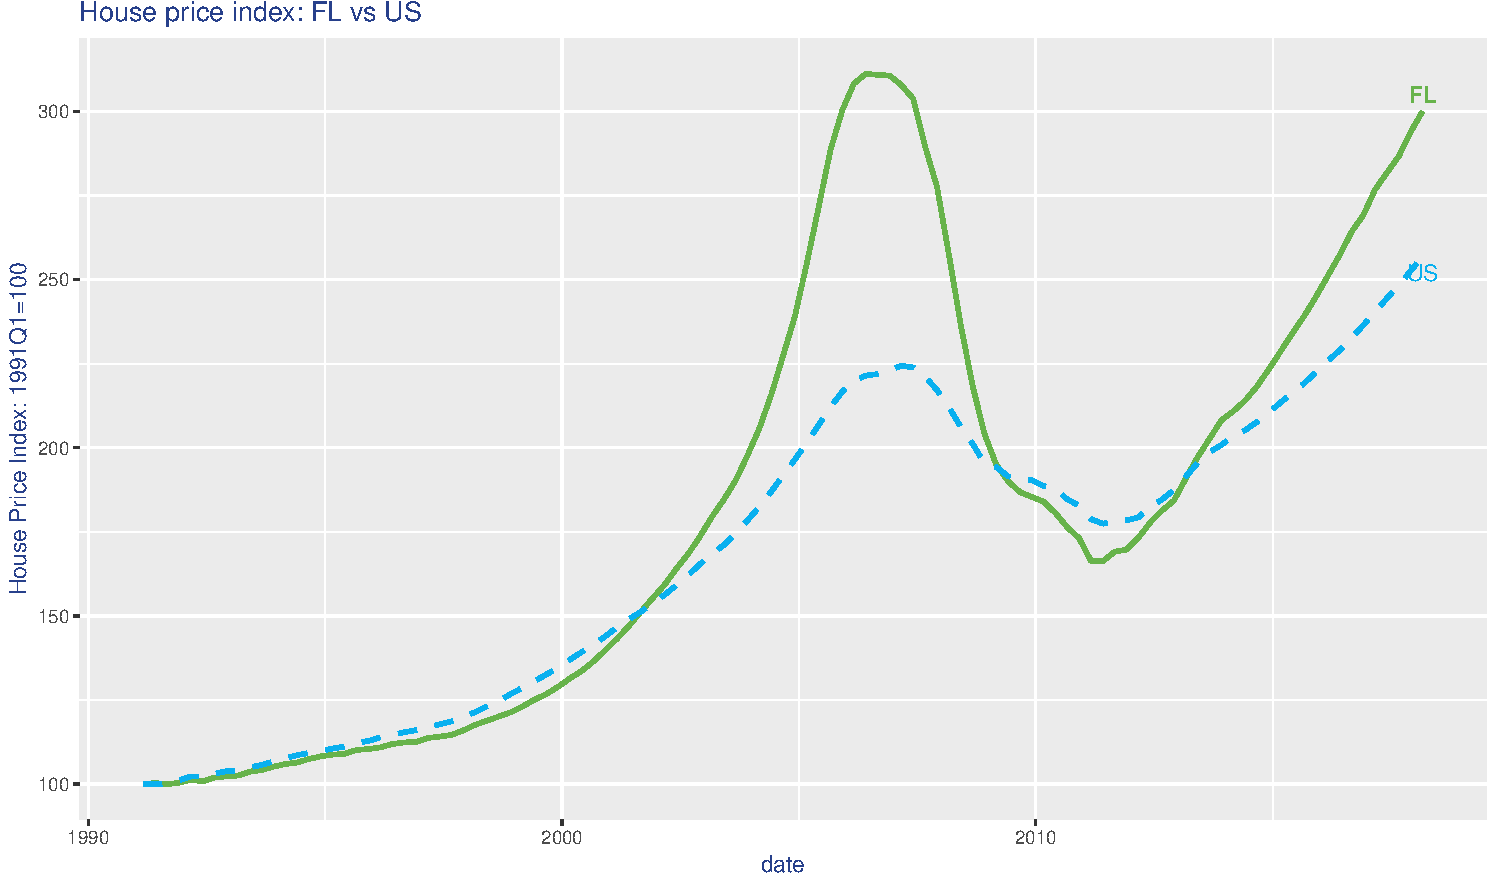
\includegraphics{Florida_pricing_files/figure-latex/query_securitization_1-1.pdf}

~ 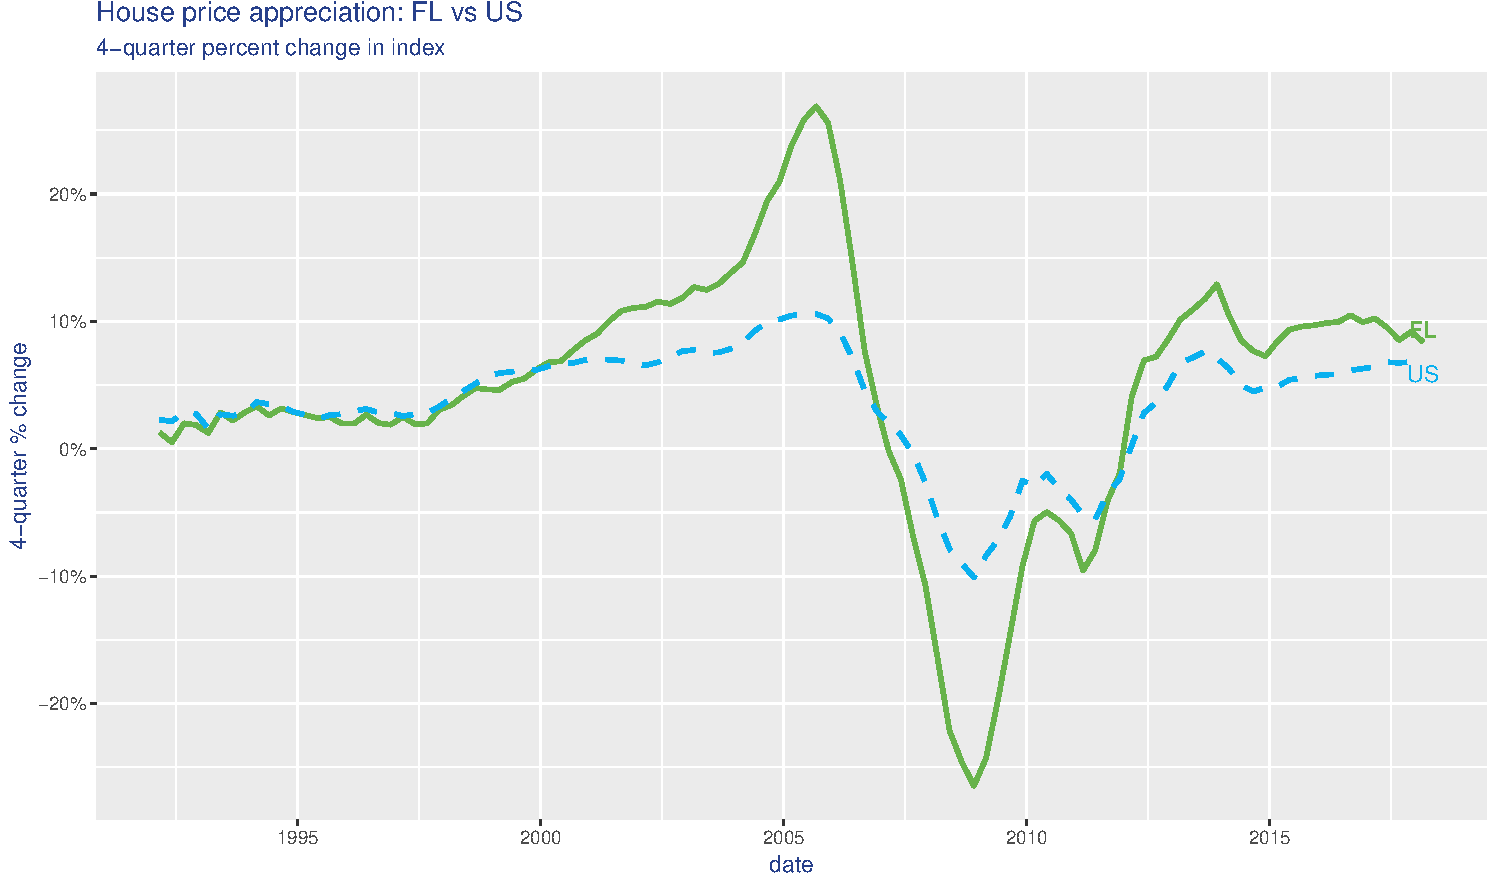
\includegraphics{Florida_pricing_files/figure-latex/loanlevel-1.pdf}
\newpage
\thispagestyle{contentpage}
\fontsize{8pt}{12pt}\selectfont\fontseries{l}

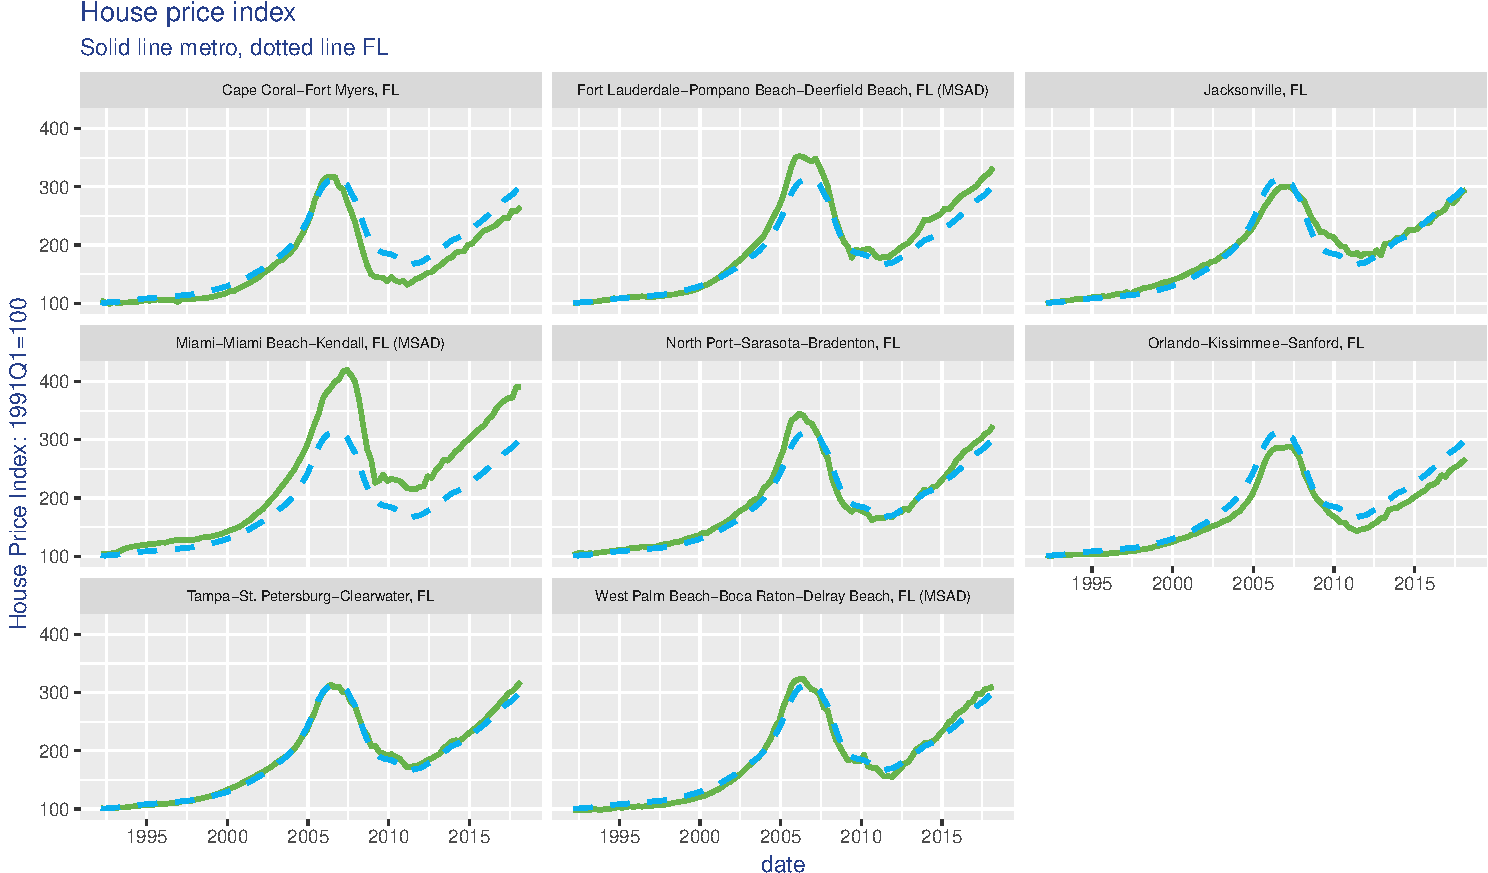
\includegraphics{Florida_pricing_files/figure-latex/AccoutLevel-1.pdf}

~

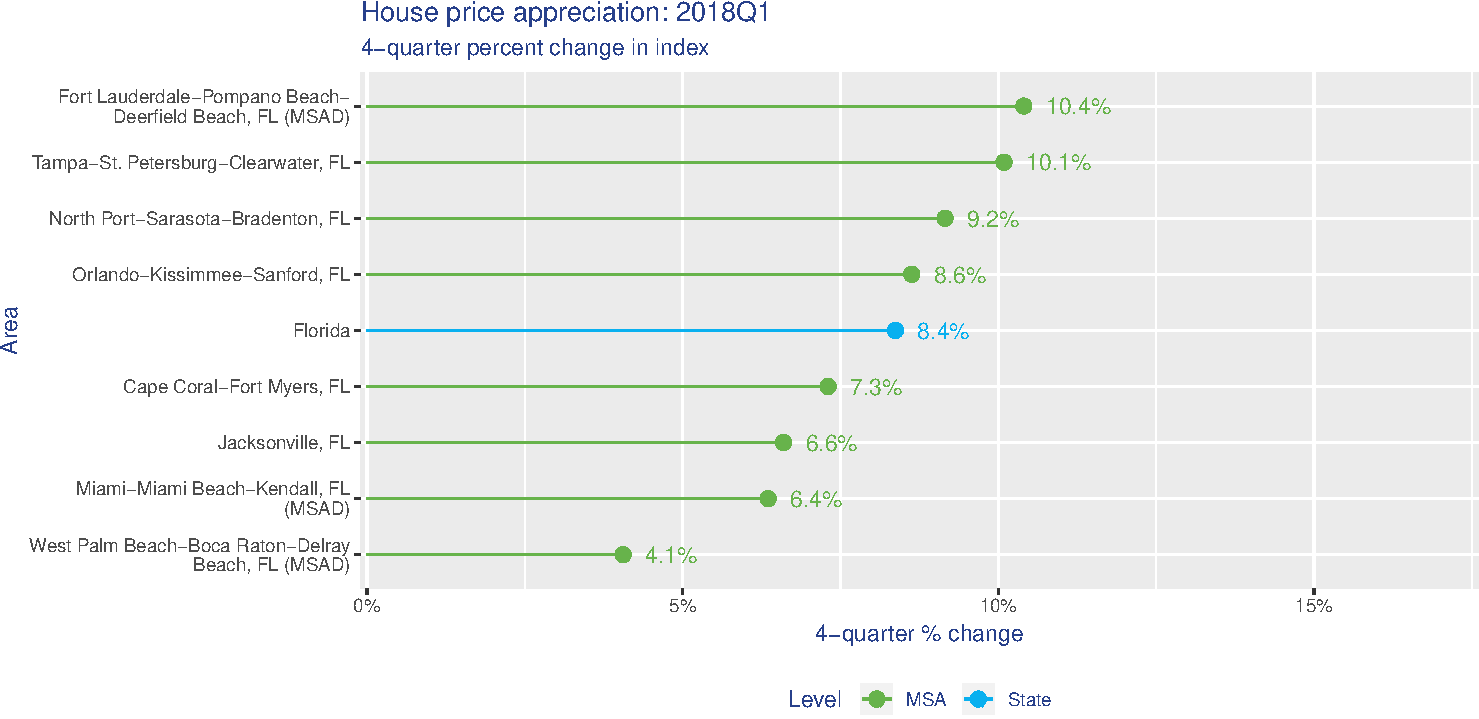
\includegraphics{Florida_pricing_files/figure-latex/MonthsOffer-1.pdf}

\newpage

\thispagestyle{contentpage}
\fontsize{8pt}{12pt}\selectfont\fontseries{l}
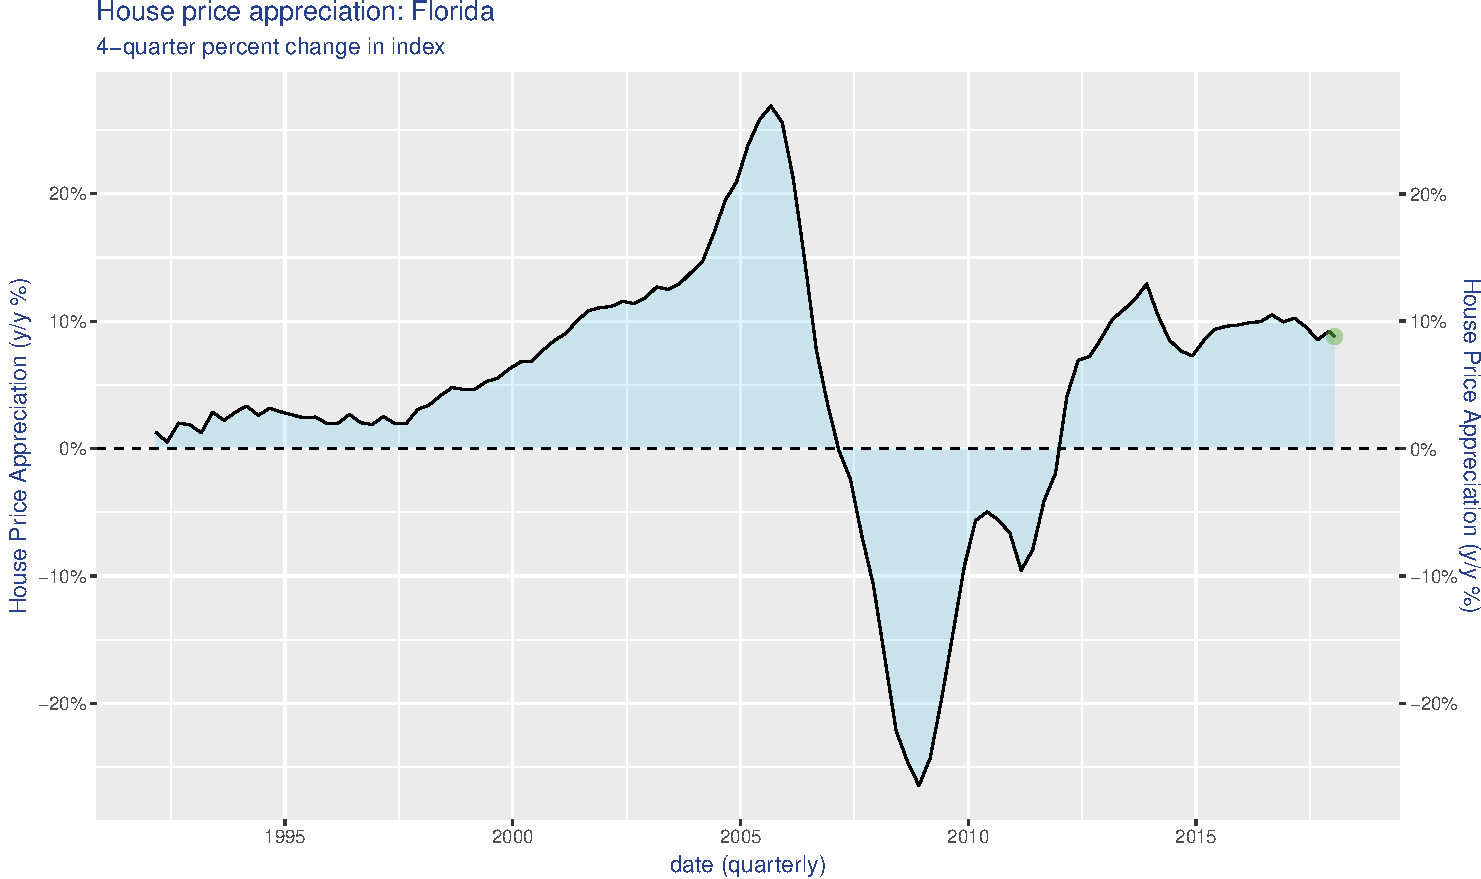
\includegraphics{Florida_pricing_files/figure-latex/MonthsOffer2-1.pdf}

\newpage

\thispagestyle{contentpage}
\fontsize{8pt}{12pt}\selectfont\fontseries{l}


\end{document}
